\documentclass[a4paper,11pt]{article}
\usepackage[utf8]{inputenc}
\usepackage[margin=1in]{geometry}
\usepackage{pdfpages}
\usepackage{mathrsfs}
\usepackage{amsfonts}
\usepackage{amsmath}
\DeclareMathOperator\arctanh{arctanh}
\usepackage{amssymb}
\usepackage{bbm}
\usepackage{amsthm}
\usepackage{graphicx}
\usepackage{centernot}
\usepackage{caption}
\usepackage{subcaption}
\usepackage{braket}
\usepackage{pgfplots}
\usepackage{lastpage}
\usepackage{enumitem}
\usepackage{setspace}
\usepackage{xcolor}
\usepackage[english]{babel} 

\usepackage[square,sort,comma,numbers]{natbib}
\usepackage[colorlinks=true,linkcolor=blue]{hyperref}

\usepackage{fancyhdr}
\newcommand{\euler}[1]{\text{e}^{#1}}
\newcommand{\Real}{\text{Re}}
\newcommand{\Imag}{\text{Im}}
\newcommand{\supp}{\text{supp}}
\newcommand{\norm}[1]{\left\lVert #1 \right\rVert}
\newcommand{\abs}[1]{\left\lvert #1 \right\rvert}
\newcommand{\floor}[1]{\left\lfloor #1 \right\rfloor}
\newcommand{\Span}[1]{\text{span}\left(#1\right)}
\newcommand{\dom}[1]{\mathscr D\left(#1\right)}
\newcommand{\Ran}[1]{\text{Ran}\left(#1\right)}
\newcommand{\conv}[1]{\text{co}\left\{#1\right\}}
\newcommand{\Ext}[1]{\text{Ext}\left\{#1\right\}}
\newcommand{\vin}{\rotatebox[origin=c]{-90}{$\in$}}
\newcommand{\interior}[1]{%
	{\kern0pt#1}^{\mathrm{o}}%
}
\newcommand*\diff{\mathop{}\!\mathrm{d}}
\newcommand{\ie}{\emph{i.e.} }
\newcommand{\eg}{\emph{e.g.} }
\newcommand{\dd}{\partial }
\newcommand{\N}{\mathbb{N}}
\newcommand{\Z}{\mathbb{Z}}
\newcommand{\R}{\mathbb{R}}
\newcommand{\C}{\mathbb{C}}
\newcommand{\w}{\mathsf{w}}

\newcommand{\Gliminf}{\Gamma\text{-}\liminf}
\newcommand{\Glimsup}{\Gamma\text{-}\limsup}
\newcommand{\Glim}{\Gamma\text{-}\lim}

\newtheorem{theorem}{Theorem}
\newtheorem{definition}{Definition}
\newtheorem{proposition}{Proposition}
\newtheorem{lemma}{Lemma}
\newtheorem{corollary}{Corollary}

\numberwithin{equation}{section}
\linespread{1.3}

\pagestyle{fancy}
\fancyhf{}
\rhead{CoCo - Assignment 1}
\lhead{}
\rfoot{\thepage}
\lfoot{Dated: \today}
\author{Johannes Agerskov, Mads Friis, and Sifan Huang}
\date{Dated: \today}
\title{CoCo - Assignment 1}
\begin{document}

	\maketitle
	
	
\section*{1.12)}
Define the language, \begin{equation}
     D=\{\omega | \omega \text{ contains an even \# of }a\text{s and an odd \# of }b\text{s and does not contain the substring }ab\}.
\end{equation}
Notice that $D=b(b^2)^*(a^2)^*$ since "does not contain $ab$ as a substring" implies $\omega\in D$ is of the form $\omega=b^ia^j$ for some $i\in2\mathbb{N}+1$ and some $j\in2\mathbb{N}$

\begin{figure}[htp]
    \centering
    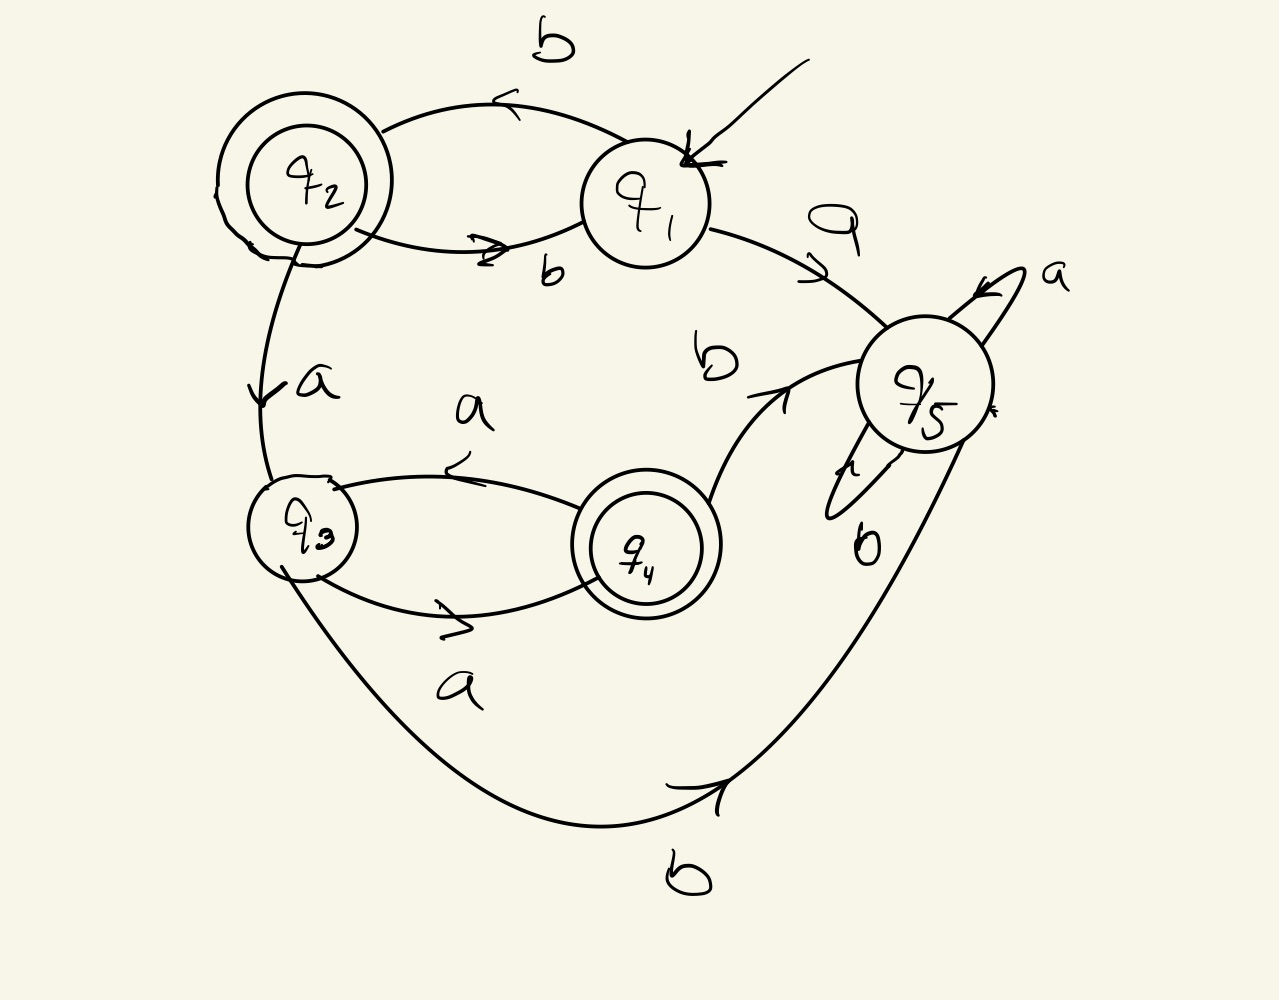
\includegraphics[width=10cm]{112.jpg}
    \caption{DFA that recognizes D}
    \label{fig:1.12}
\end{figure}
\vspace{1cm}
\pagebreak
\section*{1.16b)}
\begin{figure}[htp]
    \centering
    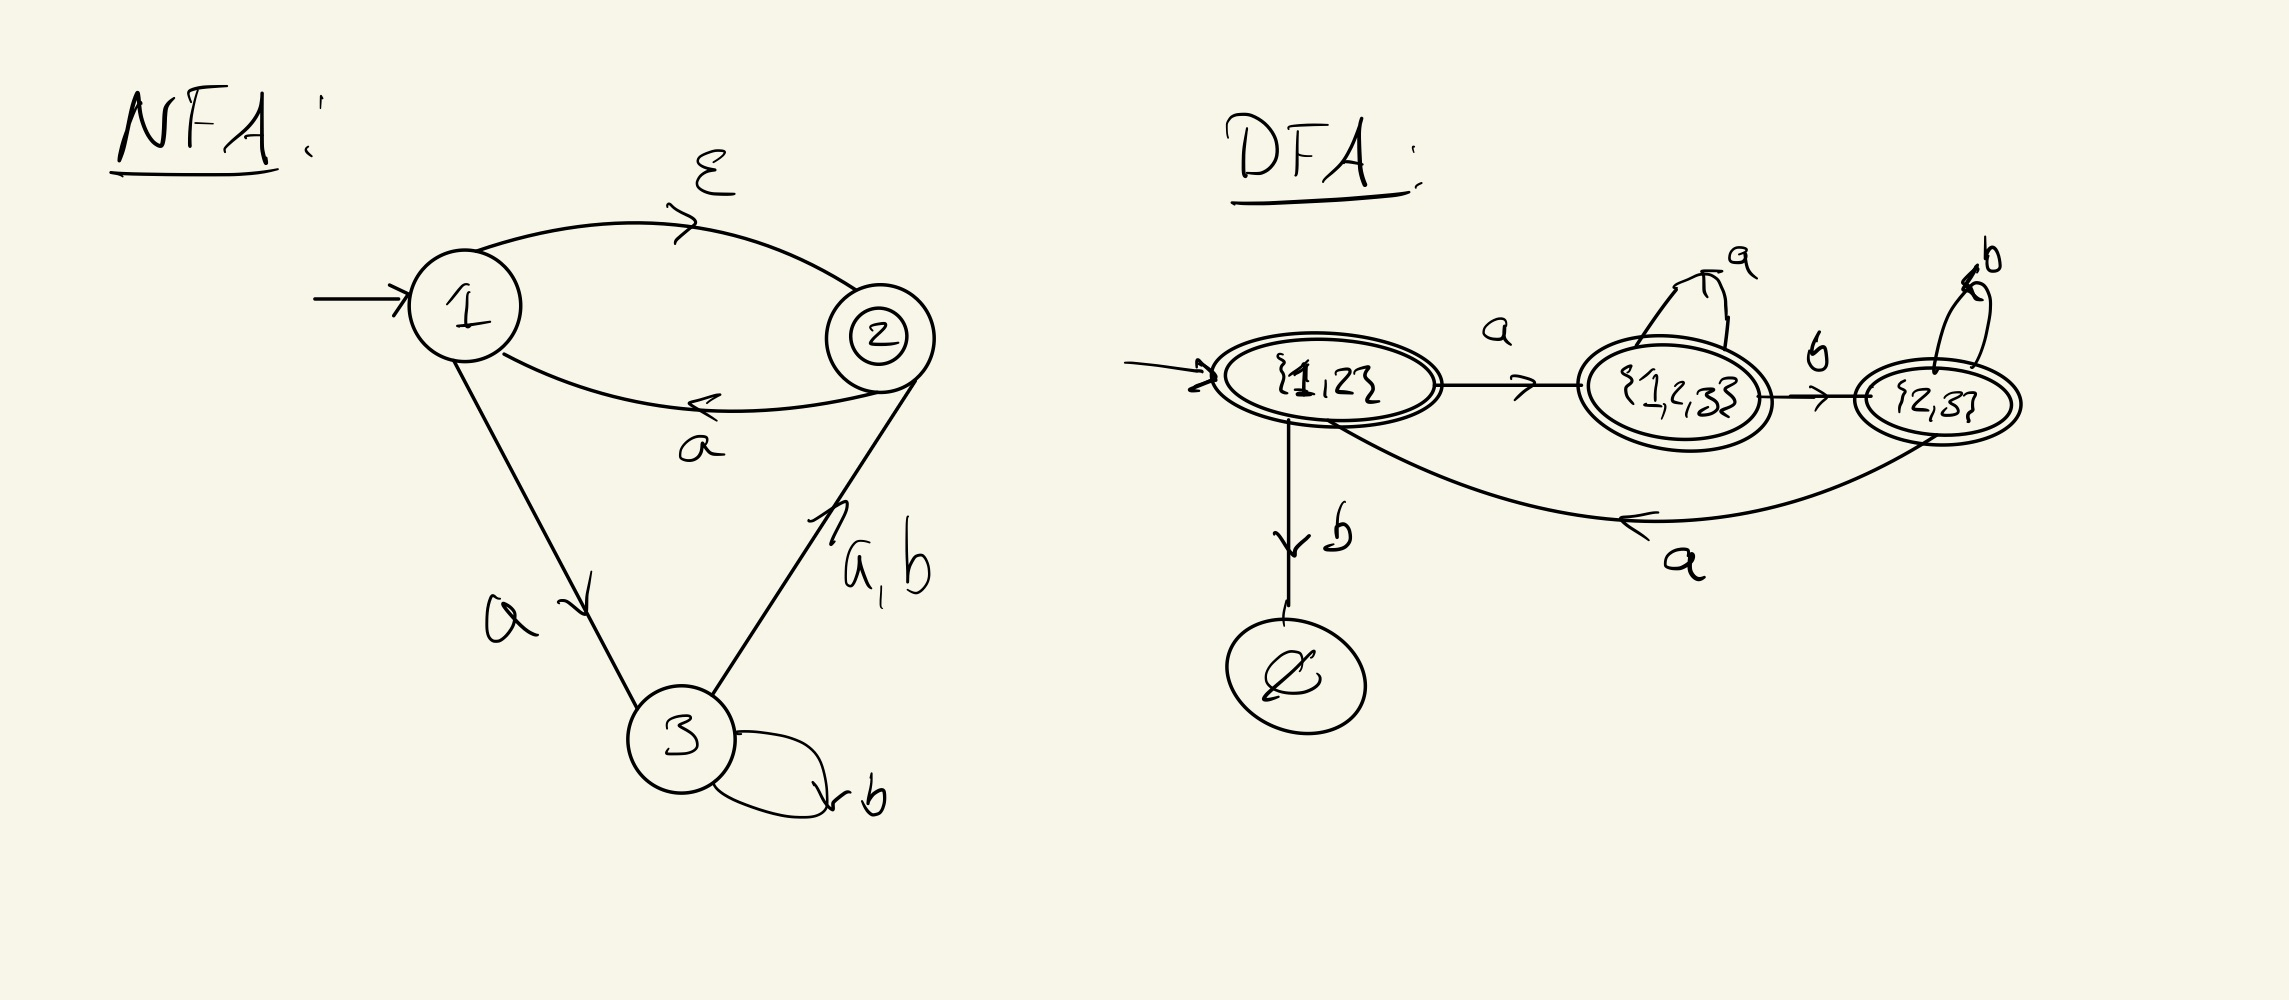
\includegraphics[width=14cm]{116.jpg}
    \caption{DFA that reckognizes the same language as the NFA given in the problem.}
    \label{fig:1.16}
\end{figure}
\vspace{1cm}
\section*{1.29)}
Show that the following languages are not regular.
\subsection*{a)}
\begin{equation}
    A_1=\{0^n1^n2^n\ \vert\ n\geq 0\}
    \end{equation}
    \begin{proof}
    Assume that $A_1$ is regular, and let $p$ be the pumping length of $A_1$. Then by the pumping lemma we known that $0^p1^p2^p$ can be split in $0^p1^p2^p=xyz$ with $\abs{y}\leq\abs{xy}\leq p$ and $\abs{y}>0$ and such that $xy^iz\in A_1$ for all $i\geq 1$. Clearly, $y=0^m$ for some $0<m\leq p$ and thus $xy^2z=0^{p+m}1^p2^p\notin A_1$. Which contradict the assumption that $A_1$ is regular.  
    \end{proof}
\subsection*{b)}
\begin{equation*}
    A_2=\{\omega\omega\omega\ \vert\ \omega\in\{a,b\}^\ast\}
\end{equation*}
    \begin{proof}
    Assume for contradiction $A_2$ is regular with pumping length $p$, and let $\omega = a^pb$. By the pumping lemma there exists $x,y,z$ such that $\omega^3 = xyz$, where $0<\abs{y}\leq \abs{xy} \leq p$. Evidently, as $\abs{xy}\leq p$, we have $y = a^l$ for some $l\geq 1$, and so $xy^2z = a^{p+l}ba^pba^pb\notin A_2$, which contradicts the pumping lemma.
    \end{proof}
\subsection*{c)}
\begin{equation*}
    A_3=\{a^{2^n}\ \vert\ n\geq 0\}
\end{equation*}
    \begin{proof}
    Assume for contradiction $A_3$ is regular with pumping length $p$, and pick some $n\in\N$ such that $p < 2^n$. By the pumping lemma there exists $x,y,z$ such that $a^{2^n} = xyz$, where $0<\abs{y}\leq\abs{xy}\leq p$. But then
    $$ 2^n < \abs{xy^2z} = 2^n + \abs{y} \leq 2^n + p < 2^{n+1}, $$
    which shows $xy^2z\notin A_3$. This contradicts the pumping lemma.
    \end{proof}


\section*{1.44)}
We construct a language that is reckognized by a DFA with $k$ states, but not any DFA with $k-1$ states. Consider the following DFA
\begin{figure}[htp]
    \centering
    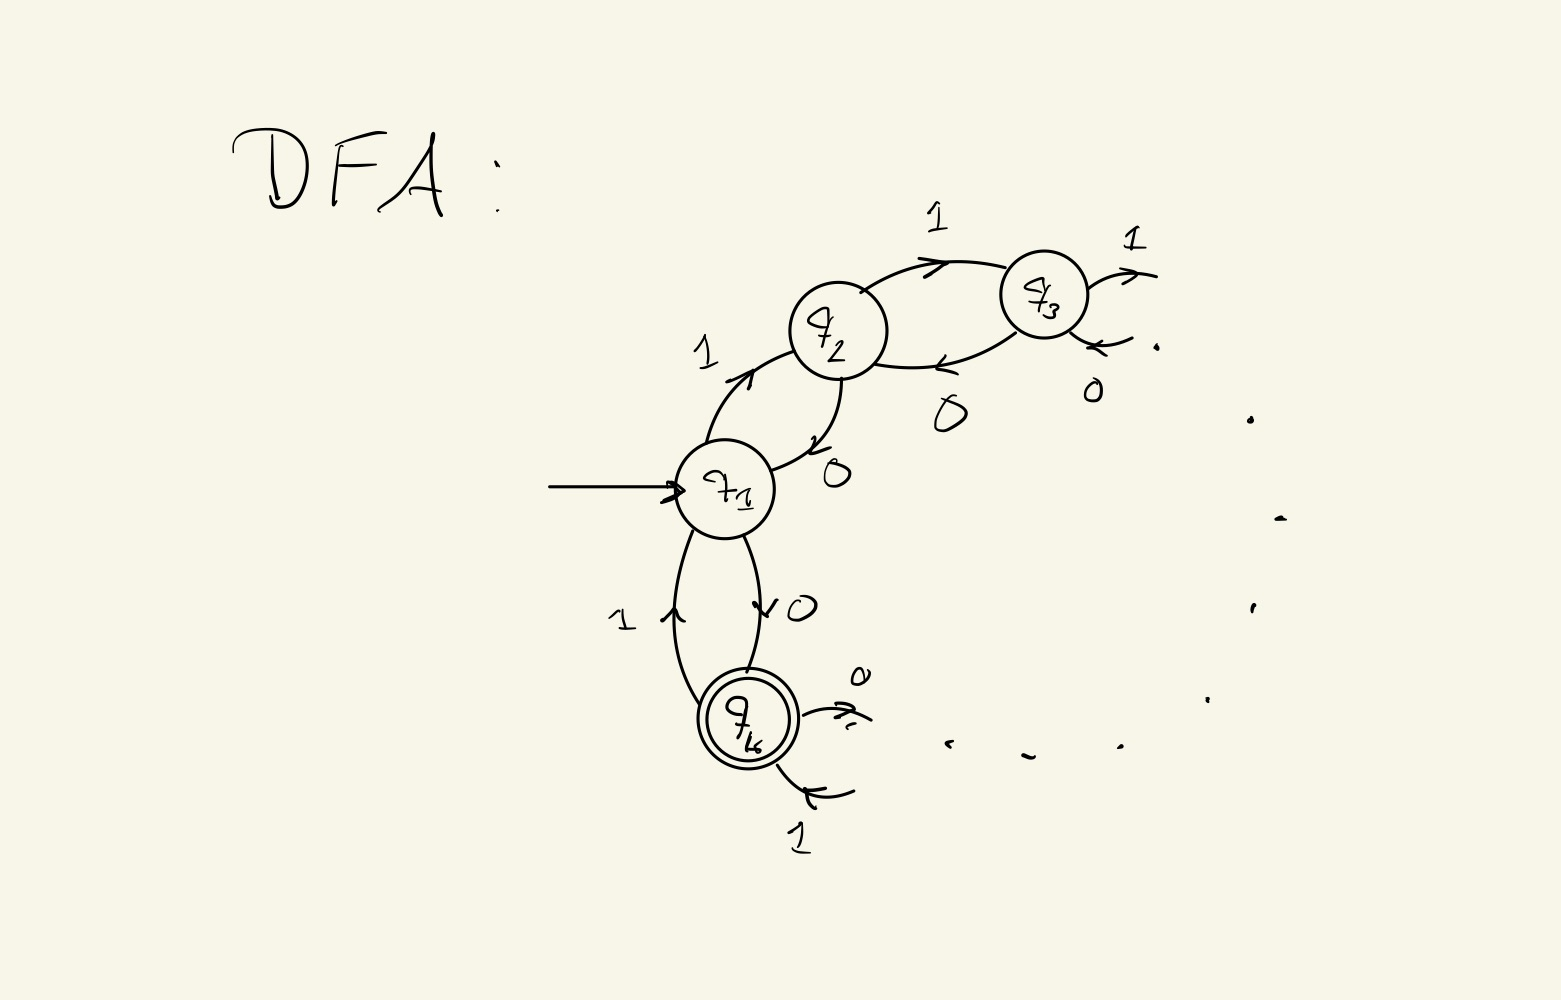
\includegraphics[width=14cm]{144.jpg}
    \caption{DFA with $k$ states.}
    \label{fig:1.44}
\end{figure}
\vspace{1cm}
This DFA reckognizes the language \begin{equation*}
    L=\{w\in\{0,1\}^\ast\ \vert\ \#1(w)-\#0(w)=k-1 \text{ mod } k\}
\end{equation*}
where $\#1(w)$ denotes the number of $1$s in $w$ and $\#0(w)$ denotes the number of $0$s in $w$. This can easily be seen by the fact that $1$s move the state clockwise and $0$s move the state counter-clockwise.
We claim that $L$ is not reckognized by any DFA with $k-1$ states.
\begin{proof}
Assume for contradiction that there exists a DFA with $k-1$ states that reckognizes $L$. Then we might, by the pumping lemma and the proof thereof, take the pumping length to be $k-1$. Now $1^{k-1}\in L$, and splitting this string according to the pumping lemma, $1^{k-1}=xyz$, we immediately conclude that $y=1^m$ for some $0<m\leq k-1$. Now clearly $xy^2z=1^{k+m-1}$ and we thus have \begin{equation*}
    \#1(xy^2z)-\#0(xy^2z)=k+m-1=m-1 \text{ mod }k<k-1\text{ mod }k.
\end{equation*}
Thereby, $xy^2z\notin L$. This contradict the fact that the pumping length can be chosen to be $k-1$, and we conclude that $L$ is not reckognized by any DFA with $k-1$ states.
\end{proof}
\section*{1.50)}
We find the minimum pumping lengths of the following languages.
\subsection*{a)}
$0001^\ast$.\\
We claim that $p_{min}=4$.
\begin{proof}
Notice that $000$ cannot be pumped, since no string contain neither more of less than three $0$s. However, any string of length $4$ or more is of the form $0001^k$ for some $k\geq1$. And clearly choosing $x=000$, $y=1$, and  $z=$"the rest", we find that $xy^iz\in 0001^\ast$ for any $i\geq0$. Thus any string of length 4 or more can be pumped.
\end{proof}
\subsection*{b)}
$0^\ast1^\ast$.\\
We claim that $p_{min}=1$.
\begin{proof}
Notice first that $p_{min}=0$ is not an option by the pumping lemma point (2), since it states that $\abs{y}>0$. However, let $w$ be any string in $0^\ast1^\ast$ with length 1 or more. Then we know that $w$ is either of the form $w=0w_0$ for some $w_0\in0^\ast1^\ast$ \emph{or} $w=w_11$ for some $w_1\in0^\ast1^\ast$. In the first case we choose $x=\varepsilon$, $y=0$, and $z=w_0$. Then $xy^iz\in0^\ast1^\ast$ for any $i\geq0$. In the second, case we choose $x=w_1$, $y=1$, and $z=\varepsilon$. Then $xy^iz\in0^\ast1^\ast$ for any $i\geq0$. Thus any string of length one or more, can be pumped.
\end{proof}
\subsection*{c)}
$L=001\cup 0^\ast1^\ast$.\\
We claim that $p_{min}=1$.
\begin{proof}
Notice that $001\in0^\ast1^\ast$, so $A=001\cup 0^\ast1^\ast= 0^\ast1^\ast$, and the rest follows from b).
\end{proof}
\subsection*{d)}
$A=0^\ast1^+0^+1^\ast\cup 10^\ast1$.
We claim that $p_{min}=3$.
\begin{proof}
Notice first that $11\in A$ cannot be pumped since for example $111\notin A$, showing that $p_{min}>2$. But if $w\in A$ with $\abs{w}\geq3$ then either $w=0...$ \emph{or} $w=11...$  \emph{or} $w=101...$ \emph{or} $w=100...$, where $"..."$ refers to "the rest of the string". In the first case we choose $x=\varepsilon$, $y=0$, and $z=...$ then we clearly have $xy^iz\in A$ for any $i\geq0$. In the second case we choose $x=\varepsilon$, $y=1$, and $z=1...$ then we clearly have $xy^iz\in A$ for any $i\geq0$. In the third case we choose $x=10$, $y=1$ and $z=...$ then we clearly have $xy^iz\in A$ for any $i\geq0$. Lastly, in the fourth case we choose $x=1$, $y=0$, and $z=0...$ then we clearly have $xy^iz\in A$ for any $i\geq0$. This proves that any string of length $3$ or more can be pumped, and thus $p_{min}\leq 3$. Combing the two bounds on $p_{min}$ shows $p_{min}=3$.
\end{proof}
\subsection*{e)}
$A=(01)^*$.
We claim that $p_{min}=1$.
\begin{proof}
Notice first that there are no string in $A$ with length 1, as all strings in $A$ have even length. Now as argued in b) the pumping length cannot be 0. So we migth start out by considering string of length 2 or more. Let $w\in A$ with $\abs{w}\geq2$, then $w=01w_0$ for some $w_0\in A$. Thus we may choose $x=\varepsilon$, $y=01$, and $z=w_0$, then clearly $xy^iz\in A$ for any $i\geq0$. This shows that any string of length 2 or more may be pumped. Now since there are no strings of length 1. It is also true that any string in $A$ of length 1 or more can be pumped, and we conclude that $p_{min}=1$.
\end{proof}
\subsection*{f)}
$A=\varepsilon$. We claim that $p_{min}=1$.
\begin{proof}
Since $p_{min}$ cannot be 0 by arguments as above in b), and since it trivially true that all strings in $A$ of length 1 or more (there are none) can be pumped, we conclude that $p_{min}=1$. Notice that this is a simple consquence of the fact that $\text{False}\implies S$ is True for any Boolean statement $S$. 
\end{proof}
\subsection*{g)}
$A=1^\ast01^\ast01^\ast$. We calin that $p_{min}=3$.
\begin{proof}
Notice first that $00$ cannot be pumped, showing that $p_{min}>2$. Now let $w\in A$ with $\abs{w}\geq3$ then either $w=1w_1$ for some $w_1\in A$ \emph{or} $w=01w_0$ for some $w_0\in1^\ast01^\ast$ \emph{or} $w=w_21$ for some $w_2\in A$. In the first case, we may choose $x=\varepsilon$, $y=1$, and $z=w_1$, then we clearly have $xy^iz\in A$ for any $i\geq0$. In the second case, we may choose $x=0$, $y=1$, and $z=w_0$, then we clearly have $xy^iz\in A$ for any $i\geq0$. In the third case, we may choose $x=w_2$, $y=1$, and $z=\varepsilon$, then we clearly have $xy^iz\in A$ for any $i\geq0$. Thus any string of length $3$ or more can be pumped, and $p_{min}\leq 3$, proving that $p_{min}=3$.
\end{proof}
\subsection*{h)}
$A=10(11^\ast0)^\ast0$
We claim that $p_{min}=4$.
\begin{proof}
Notice that $100\in A$ cannot be pumped, showing that $p_{min}>3$. This can be seen since, any downpump of $100$ will reduce the length, i.e. $xyz=100$ with $\abs{y}>0$ implies that $xy^0z=xz$ has length smaller than 3. But $100$ is clearly the shortest string in $A$ so this is not possible. However, any string in $A$ with length 5 or more may be written as $xyz$ with $x=10$, $y\in(11^\ast0)^\ast$, and $z=0$. But then $y^i\in \in(11^\ast0)^\ast$ for any $i\geq0$, showing that $xy^iz\in A$ for any $i\geq0$. Thus any string with length greater than or equal to 5 can be pumped. However, notice that $\{w\in A\ \vert\ \abs{w}=4\}=\emptyset$ so in fact any string of length 4 or more may be pumped, showing that $p_{min}=4$.
\end{proof}
\subsection*{i)}
$A=1011$. We claim that $p_{min}=5$.
\begin{proof}
Notice first that $1011$ cannot be pumped. Showing that $p_{min}>4$. However, no string in $A$ has length 5 or more, so it is true that any string in $A$ with lenght 5 or more can be pumped. Thus $p_{min}\leq5$, showing that $p_{min}=5$.
\end{proof}
\subsection*{j)}
$A=\Sigma^\ast$. We claim that $p_{min}=1$.
\begin{proof}
As before, the minimum pumping length satisfies $p_{min}\geq1$. However, for any string $w\in A$ with $\abs{w}\geq1$ we have $w=w_1s$ where $w_1$ is just the first element in $w$ and $s$ is the rest of the string, which might be the empty string. Clearly by the definition of Kleene star operation we have $w_1^is\in A$. So $w$ can be pumped, showing that $p_{min}=1$.
\end{proof}
\section*{1.53)}
Let $\Sigma=\{0,1\}$ and let $D=\{w \vert\ \#01(w)=\#10(w)\}$, where $\#s(w)$ denotes the number of occurances of the substring $s$ in $w$. We show that $D$ is a regular language\begin{proof}
We notice that $D$ can be written as a regular expression. To see this, note that the occurance of a substring $01$ is equivalent to the string switching from $0$s to $1$s and the occurance of the substring $10$ is equivalent to the string switching from $1$s to $0$s. Thus having an equal number of occurances of the two substrings means that the string starts and ends at the same letter. Therefore, $D=1\Sigma^\ast1\cup0\Sigma^\ast0$, which is a regular expression. Thus by Theorem 1.54 in M. Sipser the language is regular. 
\end{proof}
\section*{1.71)}
\subsection*{a)}
Let $B=\{1^ky\ \vert\ y\in\{0,1\}^\ast\text{ and $y$ contains at least k $1$s, for }k\geq1\}$. We show that $B$ is regular. \begin{proof}
Notice that if $w=1^ky$ for some $y\in \{0,1\}^\ast$ containing at least $k$ $1$s for some $k\geq1$. Then $w=1z$ for some $z\in \{0,1\}^\ast$ containing at least one $1$, namely $z=1^{k-1}y$ and the contrary is triavially true. Thus, if we define $\Sigma=\{0,1\}$, we clearly have $B=1\Sigma^\ast1\Sigma^\ast$, which is a regular expression. Thus by Theorem 1.54 in M. Sipser, the language is regular.
\end{proof}
\subsection*{b)}
Let $C=\{1^ky\ \vert\ y\in\{0,1\}^\ast\text{ and $y$ contains at most k $1$s, for }k\geq1\}$. We show that $C$ is not regular.
\begin{proof}
Assume for contradiction that $C$ is regular, and let $p$ be the pumping length. Then $1^p0^p1^p\in C$, and for any splitting, as described by the pumping lemma, $xyz=1^p0^p1^p$, with $\abs{xy}\leq p$ and $\abs{y}>0$ we have $y=1^m$ for some $0<m\leq p$. But then clearly $xy^0z=1^{p-m}0^p1^p$ which is \emph{not} in $C$. Since if $1^{p-m}0^p1^p=1^kw$, implies $k\leq p-m$, but clearly $w$ most contain at least $p$ $1$s then. Thus we have a contradiction with the pumping lemma, showing that $C$ is not regular.
\end{proof}
\end{document}

